\subsection{Prototypes}\label{sec:sprint2:prototypes}

At the end of Sprint 1, the existing features of \launcher were polished and the project would only need to be kept updated with the implementation of the database. \vagner{Verify that this is indeed what actually happened}
However, the Sprint 1 review meeting determined that it was desired for launcher to possibly have additional features:

\begin{itemize}
\item Selection of profiles might be desired to be selectable elsewhere in \launcher without starting an app
\item Settings for different apps could be set from an activity accessed from \launcher
\item Specification of which apps different users can access could likewise be set from an accessed from \launcher
\end{itemize}

It was decided to have a brainstorm to gather ideas regarding these features, create prototypes of the best ones\footnote{The prototypes regarded as being the best, were deemed so by the project group} and present these to the customers for feedback.

\subsubsection{Profile Selection}

At the end of Sprint 1, the profile selection would only appear when launching an app.
Two alternatives where developed:

\begin{itemize}
\item Selection of a different profile from within \launcher.
This would work by pressing the profile picture, giving a list of profiles to choose from.
Being relevant only for a guardian, the profiles selectable should only be the guardian itself and the child related to him or her.
\item Selection of a different profile from within each individual app.
While this solution does not require any modification of \launcher, it was a favourable option.
Each app would then have its own profile selection button to initiate the activities
\end{itemize}

Common for both alternatives was to display the currently selected profile in the top of the pane.
Illustrations can be seen on figure \ref{fig:profileselectionlauncherdropdown} and \ref{fig:profileselectionapppopup} respectively.

\begin{figure}[p]
    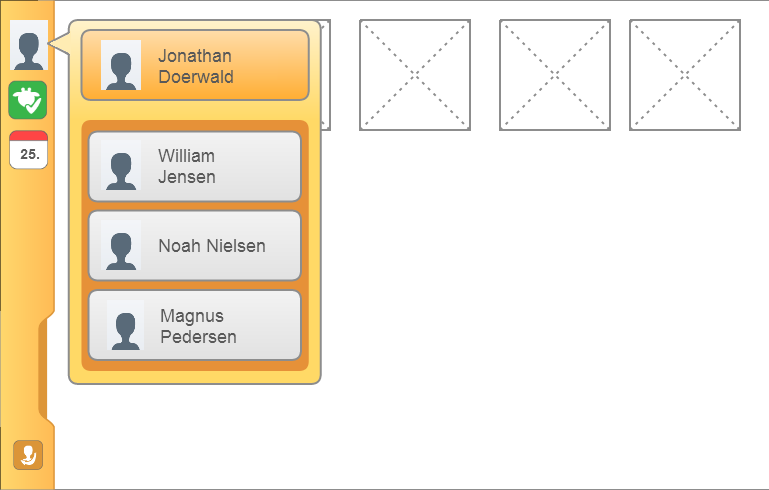
\includegraphics[width=\textwidth]{figures/sprint2/profileselectionhomescreen-dropdown}
    \caption{The dropdown profile selection option. This would appear when tapping ones profile picture as a guardian.}
    \label{fig:profileselectionlauncherdropdown}
\end{figure}

\begin{figure}[p]
    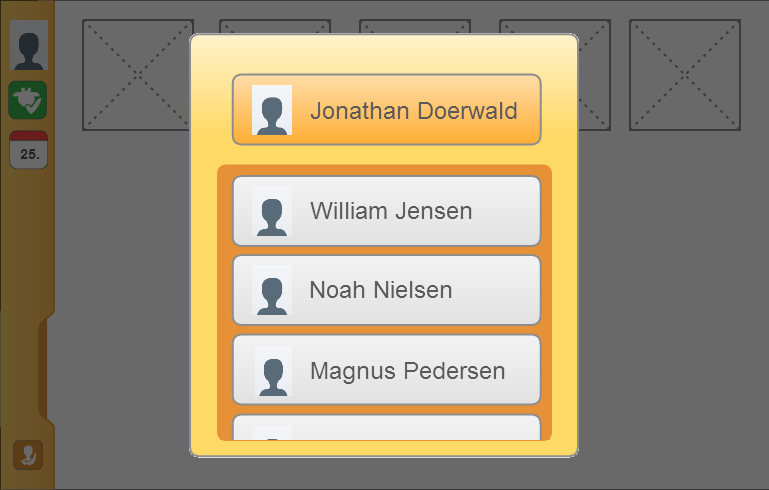
\includegraphics[width=\textwidth]{figures/sprint2/profileselection-dialog-finish}
    \caption{The profile selection pop up. These would only appear while pressing the appropiate button while inside an app.}
    \label{fig:profileselectionapppopup}
\end{figure}

\subsubsection{Settings}

At the end of sprint 1, settings for different apps where handled inside those apps exclusively.
The idea of centralizing the settings for the different apps was formed both to streamline data for the database, but also to grant the user a better overview over the settings shared by apps.

Again, two alternatives were presented:

\begin{itemize}
\item A settings app, accessible from \launcher only.
This app would contain settings for all apps enabled for the selected user, as well as selecting which apps should be enabled for that profile.
This would also include the native Android settings.
\item Letting each app have a settings button.
This would preserve the current setup.
\end{itemize}

The first option is the most encompassing one, containing functionality for both manipulate settings for other apps and decide which apps can be used with different users.
It was futhermore discussed to add functionality, allowing the user to add apps from Google Play to \launcher.
The settings part of the settings app can be seen on figure \ref{fig:settingsprototype}, while the app management part can be seen on figure \ref{}

The second option is more centered on making the settings screen streamlined across apps and would thus be a operative project with the GUI project group.
An example of settings for \launcher can e seen on figure \ref{fig:appsettingsprototype}.

\begin{figure}[p]
    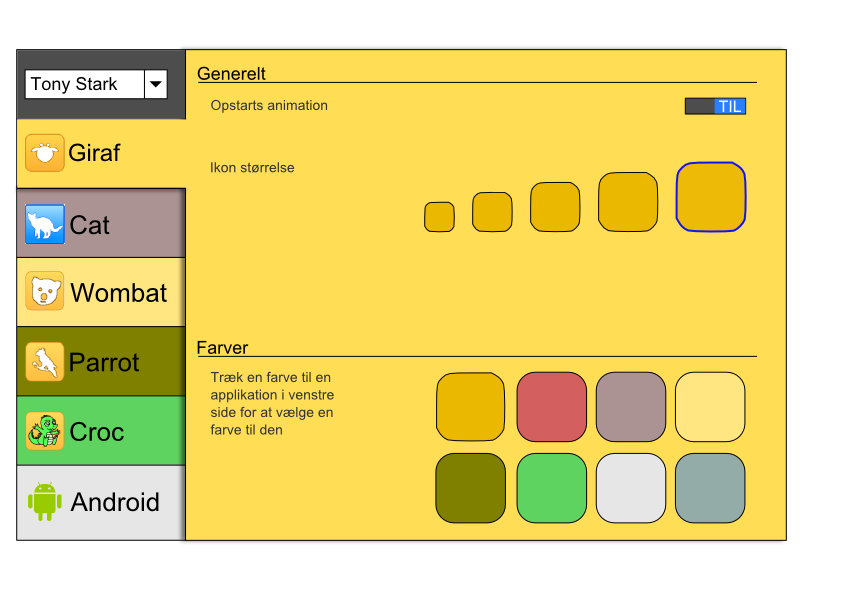
\includegraphics[width=\textwidth]{figures/sprint2/settings}
    \caption{The settings manipulation part of the settings app. in this example, settings for \launcher can be seen. The current profile being edited can be seen in the top left corner.}
    \label{fig:settingsprototype}
\end{figure}

\begin{figure}[p]
    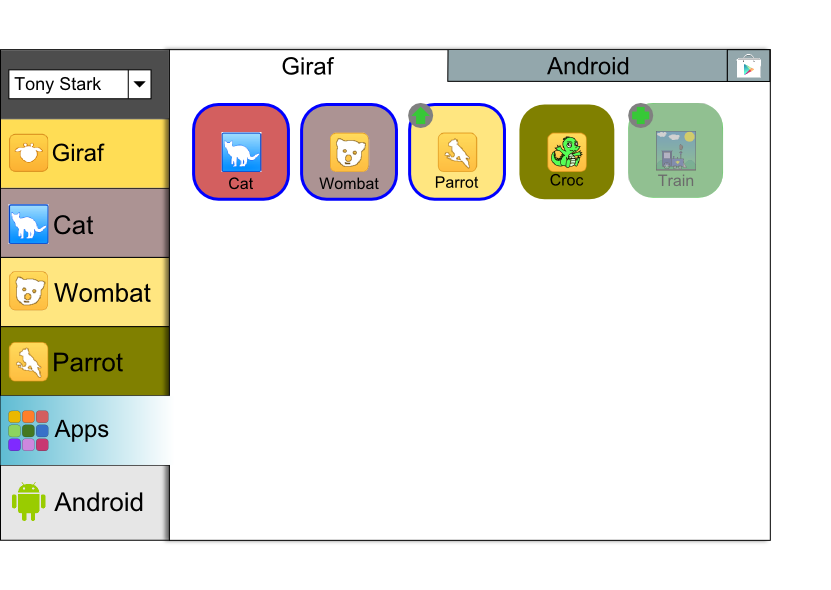
\includegraphics[width=\textwidth]{figures/sprint2/apps-colorexperiment}
    \caption{The app management part of the settings app. \giraf or Android (Google Play) apps can be choosen in the pane in the top. The current profile being edited can be seen in the top left corner}
    \label{fig:profileselectionlauncherdropdown}
\end{figure}

\begin{figure}[p]
    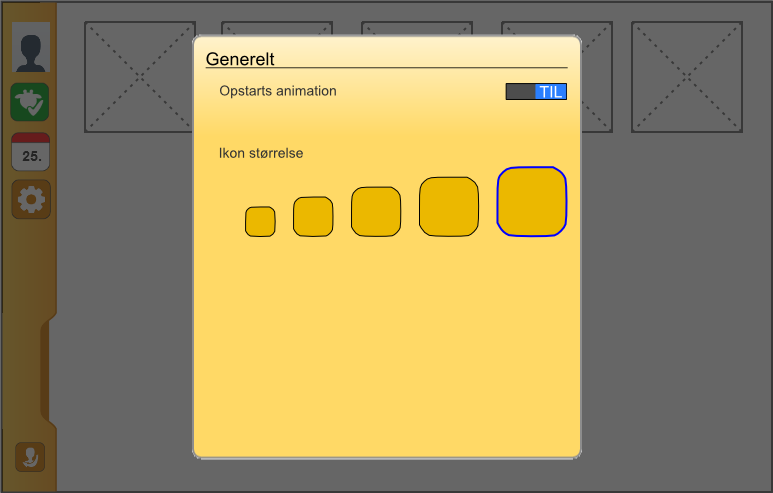
\includegraphics[width=\textwidth]{figures/sprint2/settings-dialog}
    \caption{The settings for a single app. In this example, the settings for \launcher can be seen.}
    \label{fig:appsettingsprototype}
\end{figure}

\subsubsection{Profile Info}

The group had an idea of displaying infomation about the user currently logged in in the drawer section of \launcher.
This is a relatively small feature that would be trivial to implement.
An example can be seen in figure \ref{}.

\begin{figure}[p]
    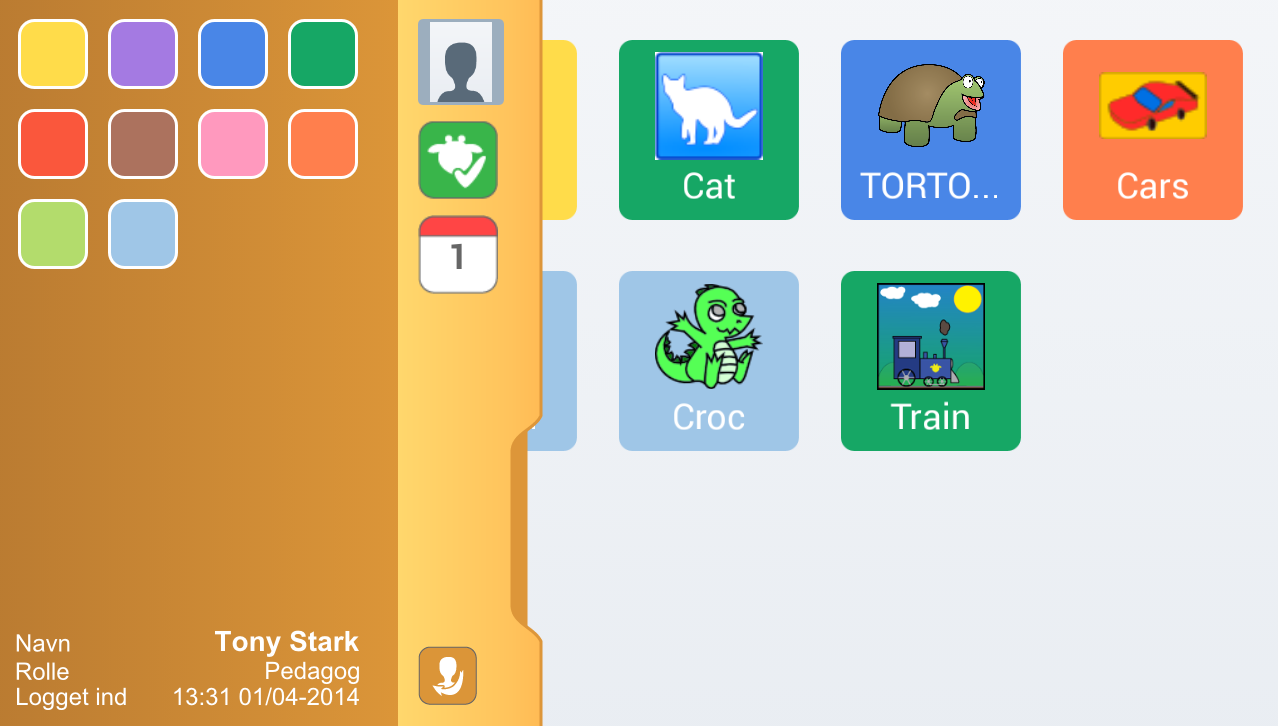
\includegraphics[width=\textwidth]{figures/sprint2/profil-info}
    \caption{An example of infomation about a user seen in the drawer.}
    \label{fig:appsettingsprototype}
\end{figure}